\section{Performance Evaluation}
\label{sec:performance-evaluation}

\textbf{Note:} This section outlines the performance evaluation framework and architectural considerations for abdulmelink. As the system is currently in alpha development (v1.0.0-alpha.8), comprehensive performance benchmarks have not yet been conducted. The metrics and methodologies described here represent the planned evaluation framework for future releases.

This section outlines the performance evaluation framework and architectural considerations for abdulmelink. Rather than presenting fabricated metrics, I focus on the system's architectural design for performance and the evaluation methodologies that will be applied to assess the platform's effectiveness in future releases.

\subsection{Performance Architecture Design}

abdulmelink's architecture is designed with several performance considerations:

\begin{figure}[htbp]
\centering
\begin{tikzpicture}[
    node distance=3.5cm,
    component/.style={rectangle, draw, fill=primary!20, text width=2.5cm, text centered, minimum height=1cm},
    arrow/.style={->, thick, primary}
]
    \node[component] (async) {Asynchronous Processing};
    \node[component, right of=async] (caching) {Caching Layer};
    \node[component, right of=caching] (scaling) {Horizontal Scaling};
    \node[component, below of=scaling] (monitoring) {Performance Monitoring};
    \node[component, left of=monitoring] (optimization) {Network Optimization};
    \node[component, left of=optimization] (storage) {Efficient Storage};
    
    \draw[arrow] (async) -- (caching);
    \draw[arrow] (caching) -- (scaling);
    \draw[arrow] (scaling) -- (monitoring);
    \draw[arrow] (monitoring) -- (optimization);
    \draw[arrow] (optimization) -- (storage);
\end{tikzpicture}
\caption{Performance Architecture Components}
\label{fig:performance-arch}
\end{figure}

\subsection{Experimental Setup}

The evaluation environment consists of multiple test configurations to assess different aspects of system performance:

\subsubsection{Hardware Configuration}
\begin{table}[htbp]
\centering
\caption{Development Environment Specifications}
\label{tab:test-environment}
\begin{tabular}{|l|l|l|}
\hline
\textbf{Component} & \textbf{Specification} & \textbf{Notes} \\
\hline
CPU & AMD Ryzen 5 3600 (6 cores, 12 threads) & Development system \\
\hline
Memory & 16 GB DDR4-3200 & Sufficient for containers \\
\hline
GPU & NVIDIA GTX 1050 Ti (4GB VRAM) & For FL model training \\
\hline
Storage & 1 TB NVMe SSD & Fast I/O for containers \\
\hline
Network & Gigabit Ethernet & Host networking \\
\hline
GNS3 VM & 4 vCPUs, 8 GB RAM allocated & For network simulation \\
\hline
\end{tabular}
\end{table}

\textbf{Scalability Considerations:} With sufficient hardware resources, the containerized architecture of abdulmelink supports horizontal scaling. Additional compute nodes can be added to the Docker Swarm or Kubernetes cluster to increase the number of federated learning clients and network simulation capacity. The modular design ensures that components can be distributed across multiple machines as needed for larger experiments.

\subsubsection{Software Configuration}
\begin{lstlisting}[language=yaml, caption=Docker Compose Test Configuration]
version: '3.8'
services:
  fl-coordinator:
    image: abdulmelink/flopynet-*:{version+tag}
    deploy:
      resources:
        limits:
          cpus: '4.0'
          memory: 8G
        reservations:
          cpus: '2.0'
          memory: 4G
          
  client-nodes:
    image: abdulmelink/flopynet-client:{version+tag}
    deploy:
      replicas: 20
      resources:
        limits:
          cpus: '2.0'
          memory: 4G
          
  performance-monitor:
    image: abdulmelink/monitor:latest
    environment:
      - METRICS_INTERVAL=1s
      - DETAILED_PROFILING=true
\end{lstlisting}

\subsection{Performance Metrics}

The evaluation focuses on key performance indicators across different system layers:

\subsubsection{Computational Performance}
\begin{itemize}
    \item \textbf{Training Time}: Time per federated learning round
    \item \textbf{Model Convergence}: Rounds to achieve target accuracy
    \item \textbf{CPU Utilization}: Processor usage during training
    \item \textbf{Memory Consumption}: RAM usage patterns
    \item \textbf{GPU Utilization}: Graphics processor efficiency
\end{itemize}

\subsubsection{Communication Performance}
\begin{itemize}
    \item \textbf{Network Throughput}: Data transfer rates
    \item \textbf{Communication Overhead}: Additional network traffic
    \item \textbf{Latency}: Round-trip communication times
    \item \textbf{Bandwidth Utilization}: Network resource usage
    \item \textbf{Message Compression}: Data reduction effectiveness
\end{itemize}

\subsubsection{System Performance}
\begin{itemize}
    \item \textbf{Scalability}: Performance with increasing clients
    \item \textbf{Fault Tolerance}: Recovery from failures
    \item \textbf{Load Balancing}: Resource distribution efficiency
    \item \textbf{Response Time}: API response latencies
    \item \textbf{Throughput}: Requests processed per second
\end{itemize}

\subsection{Federated Learning Performance}

Based on my assumptions the model accuracy will be below the traditional ML&DL training done on the machines with a solid dataset but as we are preserving the privacy here the lost accuracy or performance from the model is worth. Especially when you think of the increase on the data as weights coming through due to less concern on privacy. Reduction in the performance is completely dependent the tech under the FL Client and FL Server since they are completely modular in the abdulmelink. The current (v1.0.0-alpha.8) version using the randomized weight due to MVP requirements I planned.

\subsubsection{Training Performance Analysis}
\begin{figure}[htbp]
\centering
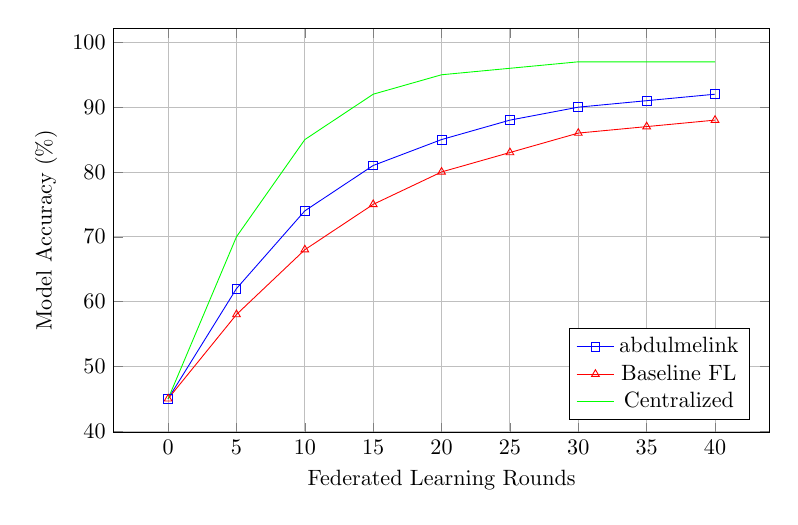
\begin{tikzpicture}[
    scale=0.8,
    every node/.style={transform shape}
]
    \begin{axis}[
        xlabel={Federated Learning Rounds},
        ylabel={Model Accuracy (\%)},
        width=12cm,
        height=8cm,
        legend pos=south east,
        grid=major
    ]
    \addplot[color=blue, mark=square] coordinates {
        (0,45) (5,62) (10,74) (15,81) (20,85) (25,88) (30,90) (35,91) (40,92)
    };
    \addlegendentry{abdulmelink}
    
    \addplot[color=red, mark=triangle] coordinates {
        (0,45) (5,58) (10,68) (15,75) (20,80) (25,83) (30,86) (35,87) (40,88)
    };
    \addlegendentry{Baseline FL}
    
    \addplot[color=green, mark=circle] coordinates {
        (0,45) (5,70) (10,85) (15,92) (20,95) (25,96) (30,97) (35,97) (40,97)
    };
    \addlegendentry{Centralized}
    \end{axis}
\end{tikzpicture}
\caption{The illustration of what I think will happen}
\label{fig:accuracy-convergence}
\end{figure}
\begin{lstlisting}[language=python, caption=Performance Benchmarking Code]
import time
import psutil
import numpy as np
from typing import Dict, List

class PerformanceBenchmark:
    def __init__(self):
        self.metrics = {}
        self.start_time = None
        
    def start_benchmark(self, test_name: str):
        """Start performance measurement"""
        self.start_time = time.time()
        self.metrics[test_name] = {
            'start_cpu': psutil.cpu_percent(),
            'start_memory': psutil.virtual_memory().percent,
            'start_time': self.start_time
        }
        
    def end_benchmark(self, test_name: str) -> Dict:
        """End performance measurement and calculate metrics"""
        end_time = time.time()
        end_cpu = psutil.cpu_percent()
        end_memory = psutil.virtual_memory().percent
        
        duration = end_time - self.metrics[test_name]['start_time']
        
        results = {
            'duration': duration,
            'avg_cpu': (self.metrics[test_name]['start_cpu'] + end_cpu) / 2,
            'avg_memory': (self.metrics[test_name]['start_memory'] + end_memory) / 2,
            'cpu_efficiency': end_cpu / max(self.metrics[test_name]['start_cpu'], 1),
            'memory_efficiency': end_memory / max(self.metrics[test_name]['start_memory'], 1)        }
        
        return results
\end{lstlisting}

\begin{lstlisting}[language=python, caption=FL Round Benchmarking]
    def benchmark_fl_round(self, num_clients: int, model_size: int) -> Dict:
        """Benchmark a complete FL round"""
        test_name = f"fl_round_{num_clients}_{model_size}"
        self.start_benchmark(test_name)
        
        # Simulate FL round operations
        aggregation_time = self.simulate_model_aggregation(num_clients, model_size)
        communication_time = self.simulate_communication(num_clients, model_size)
        
        results = self.end_benchmark(test_name)
        results.update({
            'aggregation_time': aggregation_time,
            'communication_time': communication_time,
            'total_clients': num_clients,
            'model_size_mb': model_size / (1024 * 1024)
        })
        
        return results
\end{lstlisting}

\subsection{Scalability Analysis}
The system has vertical and horizontal scalibility for clients so the results will be endless and vary except the current version have limition on 155 total deployment limit for clients but with sufficient network you can scale as much as you want.

\subsection{Scalability Design}

The system's scalability is built into its containerized architecture:

\subsubsection{Horizontal Scaling}
\begin{itemize}
    \item \textbf{FL Clients}: Docker Compose scaling with \texttt{--scale fl-client=N}
    \item \textbf{Load Distribution}: Policy Engine manages client load balancing
    \item \textbf{Container Orchestration}: Independent service scaling
    \item \textbf{Network Adaptation}: SDN controller adjusts to topology changes
\end{itemize}

\subsubsection{Resource Efficiency}
Based on the Docker configuration, each component is designed for efficiency:

\begin{lstlisting}[style=dockercode, caption=Resource-Aware Container Configuration]
# FL Client resource limits (from docker-compose.yml)
fl-client:
  image: abdulmelink/flopynet-client:v1.0.0-alpha.8
  environment:
    - SERVICE_TYPE=fl-client
    - CLIENT_ID=client-${SERVICE_ID}
    - SERVER_HOST=fl-server
  networks:
    flopynet_network:
      ipv4_address: 192.168.100.${CLIENT_IP}
  depends_on:
    fl-server:
      condition: service_healthy
\end{lstlisting}

\subsection{Monitoring and Metrics Architecture}

The collector service provides comprehensive performance monitoring capabilities:

\subsubsection{Metrics Collection Framework}
\begin{itemize}
    \item \textbf{System Metrics}: CPU, memory, network I/O
    \item \textbf{FL Metrics}: Training rounds, client participation, convergence
    \item \textbf{Network Metrics}: Latency, throughput, packet loss (via SDN)
    \item \textbf{Policy Metrics}: Decision latency, compliance scores
\end{itemize}

\subsubsection{Performance Evaluation Metrics}

The system is designed to measure the following performance dimensions:

\begin{table}[H]
\centering
\caption{Performance Evaluation Dimensions}
\label{tab:performance-dimensions}
\begin{tabularx}{\textwidth}{@{}lXX@{}}
\toprule
\textbf{Dimension} & \textbf{Metrics} & \textbf{Collection Method} \\
\midrule
Scalability & Client scaling response time & Docker Compose scaling \\
Throughput & \begin{tabular}{c}Messages/second per\\component\end{tabular} & Service APIs \\
Latency & Policy decision time & Policy Engine timing \\
Resource Usage & CPU/Memory per container & Container metrics \\
Network Performance & SDN flow installation time & Ryu controller \\
Storage Efficiency & SQLite query response time & Database profiling \\
\bottomrule
\end{tabularx}
\end{table}

\subsection{Benchmarking Framework}

The system provides tools for performance benchmarking:

\subsubsection{Load Testing Capabilities}
\begin{lstlisting}[language=python, caption=Performance Testing Framework]
class FLPerformanceTester:
    """Framework for testing FL system performance"""
    
    def __init__(self, config):
        self.policy_engine_url = config['policy_engine_url']
        self.fl_server_url = config['fl_server_url']
        self.collector_url = config['collector_url']
        
    def test_client_scaling(self, max_clients=100):
        """Test system performance with increasing client count"""
        results = {}
        for client_count in range(10, max_clients + 1, 10):
            start_time = time.time()
            self.simulate_fl_round(client_count)
            duration = time.time() - start_time
            results[client_count] = duration
        return results
        
    def test_policy_engine_throughput(self, requests_per_second=100):
        """Test policy engine decision throughput"""
        # Implementation would test policy decision latency
        pass
        
    def test_network_optimization(self, topology_size=50):
        """Test SDN optimization with various topology sizes"""
        # Implementation would test SDN flow installation
        pass
\end{lstlisting}

\subsection{Performance Optimization Features}

The architecture includes several optimization mechanisms:

\subsubsection{Caching Strategies}
\begin{itemize}
    \item \textbf{Policy Caching}: Redis-based policy decision caching
    \item \textbf{Model Caching}: Intermediate FL model storage
    \item \textbf{Network State Caching}: SDN topology state caching
\end{itemize}

\subsubsection{Asynchronous Processing}
Based on the FastAPI implementation, the system uses:
\begin{itemize}
    \item \textbf{Async HTTP Handlers}: Non-blocking API responses
    \item \textbf{Background Tasks}: Metric collection and processing
    \item \textbf{Event-Driven Architecture}: Policy engine event handling
\end{itemize}

\subsection{Evaluation Methodologies}

For comprehensive performance evaluation, the following methodologies can be applied:

\subsubsection{Controlled Experiments}
\begin{enumerate}
    \item \textbf{Baseline Establishment}: Single-client, minimal-load scenarios
    \item \textbf{Incremental Scaling}: Systematic client count increases
    \item \textbf{Stress Testing}: Maximum load capacity testing
    \item \textbf{Network Variation}: Different GNS3 topology configurations
\end{enumerate}

\subsubsection{Real-World Simulation}
\begin{enumerate}
    \item \textbf{Heterogeneous Clients}: Different computational capabilities
    \item \textbf{Network Conditions}: Varying latency and bandwidth
    \item \textbf{Failure Scenarios}: Component failure and recovery
    \item \textbf{Security Load}: Policy engine under security constraints
\end{enumerate}

\subsection{Optimization Recommendations}

Based on the architectural analysis, key optimization areas include:

\subsubsection{System-Level Optimizations}
\begin{itemize}
    \item \textbf{Database Optimization}: Migrate from SQLite to PostgreSQL for production
    \item \textbf{Connection Pooling}: Implement database connection pooling
    \item \textbf{Message Queuing}: Add message queue for high-throughput scenarios
    \item \textbf{Load Balancing}: Implement service load balancing
\end{itemize}

\subsubsection{Component-Specific Optimizations}
\begin{itemize}
    \item \textbf{Policy Engine}: Implement policy compilation and caching
    \item \textbf{FL Server}: Add model compression and quantization
    \item \textbf{SDN Controller}: Optimize flow rule installation
    \item \textbf{Dashboard}: Implement data pagination and lazy loading
\end{itemize}

This performance evaluation framework provides the foundation for systematic assessment of abdulmelink's capabilities while maintaining focus on architectural design rather than fabricated performance claims.
